\documentclass{article}

\linespread{1.5}
\usepackage[utf8]{inputenc}
\usepackage[left=1.5in,right=1.5in,bottom=1in]{geometry}
\setlength\parindent{0pt}
\setlength{\parskip}{1em}
\setcounter{secnumdepth}{0}
\usepackage{outlines}
\usepackage{graphicx}
\graphicspath{ {imgs} }
\usepackage[hyphens]{url}
\usepackage{hyperref}
\usepackage{color,soul}
\usepackage[normalem]{ulem}

\usepackage[
backend=biber,
style=apa,
citestyle=authoryear,
sorting=nyt,
]{biblatex}
\addbibresource{refs.bib}

\usepackage{comment}
\specialcomment{topicsen}{\begingroup\bfseries\scriptsize}{\endgroup}
%\excludecomment{topicsen}

\newcommand{\alignedmarginpar}[1]{%
        \marginpar{\raggedright\small #1}
    }

\title{Spring School}
\author{Carla Hyenne}

\begin{document}

\maketitle

\tableofcontents

\pagebreak

\section{Readings}


Williams, J. (2021).  (1st ed.). Routledge, 8–18. https://doi.org/10.4324/9780429490613.

\subsubsection{\textit{Moving from a circular economy to a circular city, in: Circular Cities: A Revolution in Urban Sustainability}, Jo Williams, 2021}

\begin{outline}
	\1 Circularity is an ecological concepts, where resources are recycled, reused or recovered. Used in industrial systems, production processes (cradle to cradle), and economic systems (circular economy) but none of these have focused on \textit{urban systems} as an area for analysis 
	\1 ``Circular economy is a model for production and consumption (with an emphasis on production), whose ultimate goal is to achieve the decoupling of economic growth form natural resource depletion and environmental degradation'' (p. 9)
		\2 Circular economy designs regeneration and restoration (of the previous damage) into economic processes
		\2 RESOLVE is the most use framework for circular economy in businesses, but not so applicable for the circular city
	\1 Economic vs. Urban system - the differences: (p. 11)
		\2 Governed at national and international levels vs. spatially bounded, governed at local level although affected by national and international `regulatory and economic systems'
		\2 Goals are economic, accumulation of wealth and capital vs. goals are about societal benefits
		\2 Focus on businesses or industries vs. focus on systems of production
		\2 RESOLVE doesn't consider that:
			\3 Cities are often centres of consumption, not production, which happens outside the city; the `waste' produced in the city is thus mostly individual waste, not industrial
			\3 Cities have many different groups of people, with different social practices, and are highly complex social spaces
			\3 Scale:  important to consider at which scale to intervene, neighbourhood, city, city region?
	\1 Moving from an economic to ecological focus
		\2 Ecological footprint: the area of land and water required to produce the resources (goods and services) necessary for the urban system to function well (food, energy,...); it is located outside the city boundaries, and the goal of a city should be to minimise this area; Need to reduce: resources consumed AND waste generated
		\2 Sufficiency: self-sufficiency to increase resilience 
		\2 Closing resource loops: reducing inefficiencies by closing resource loop, and reusing, reducing, recovering
		\2 Regenerative capacity: capacity to produce resources and absorb waste does not function well, and cities have to rely on increasingly larger hinterlands to sustain their population
		\2 Adaptive capacity: ``socio-technical lock-ins to existing infrastructure and land-use patterns'' prevents resources from being fully utilised, and creates waste in cities 
		\2 Context: local politics influence all of the above
	\1 ``A circular city is a socio-ecological system, consisting of a bio-geo-physical unit and its associated social actors and institutions. It is a complex, regenerative and adaptive system, delimited by spatial and functional boundaries, surrounding an ecosystem.'' (p. 15). Three actions for circular city and development, to operate within \textbf{ecological carrying capacity}:
		\2 Looping actions: from a linear to a closed process
		\2 Ecologically regenerative actions: integrating blue and green spaces into urban fabric/management of urban ecosystem
		\2 Adaptive actions: capacity within the urban fabric to adapt to change
	\1 ``A variety of circular development pathways are likely to emerge from different urban contexts, resulting from diverse political economic, cultural, social, environmental, regulatory and technical conditions'' (p. 15)
	\1 Varying motivations for a circular city: city-marketing, exporting urban innovation, social solidarity and redistribution of resources, business development and job creation, regenerating local industry base, resource security, climate change... 
\end{outline}

\subsubsection{\textit{Circular economy and the city: an urban political economy agenda}, Keblowski, W., Lambert, D. \& Bassens, D, 2020}

\begin{outline}
	\1 
\end{outline}

\subsubsection{\textit{Exploring circular economies in the built environment from a complex systems perspective}, Rios et al., 2022}

\begin{outline}
	\1 
\end{outline}

\subsubsection{\textit{Downscaling the Doughnut to the City}, Kate Raworth, 2021}

\url{https://www.youtube.com/watch?v=YCqGf7T9ABoLink/URL}

\begin{outline}
	\1 How can the city meet the needs of its people, so that they thrive (including food, housing, health care, education, transport, political voice, social equality) without compromising the needs of the planet? What does that look like for your city, given its geography and environmental boundaries? $\rightarrow$ \textbf{thriving people in a thriving habitat}
	\1	Experiments conducted in Portland, Philadelphia, Amsterdam, downscaling the doughnut into a `city portrait'
		\2 Amsterdam's housing: unaffordable, but housing cannot continue to be built in the same way it has been, if it is to be sustainable and respect the environment? How can housing be circular, incl. material waste, energy usage, land use, biodiversity,... 
	\1 The role of individuals to tell their stories and lived experiences (`city selfie')
\end{outline}

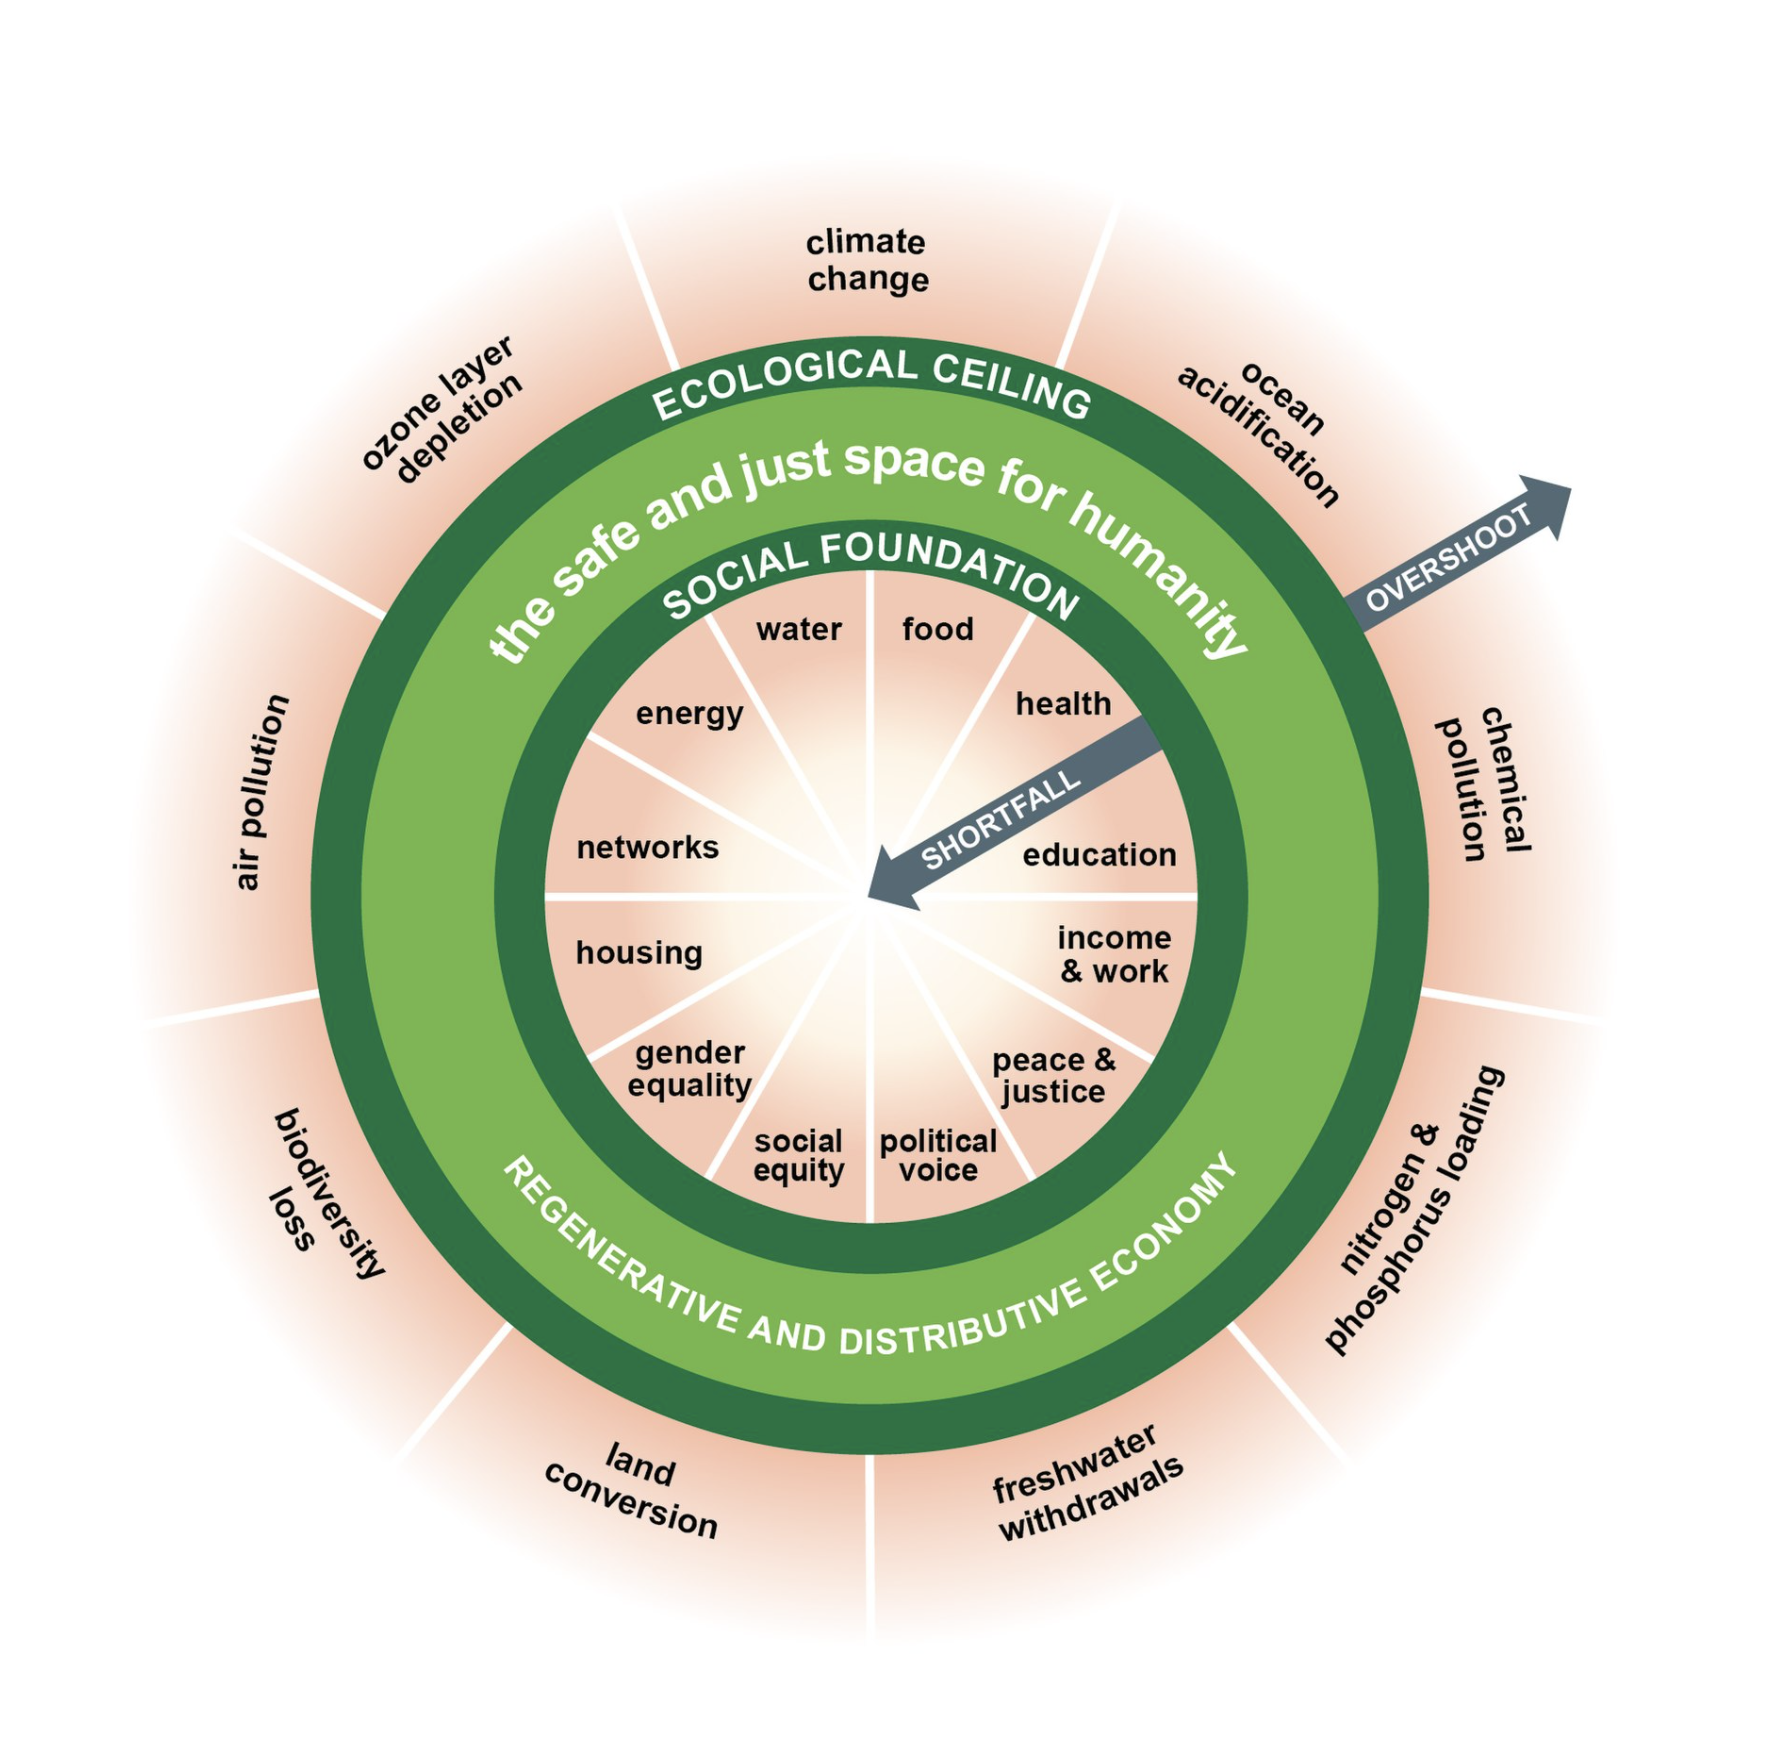
\includegraphics[width=\textwidth]{doughnut_economics}

\printbibliography

\end{document}

